\chapter{Estudo de Caso} \label{estudodecaso}

\section{Definição} \label{definicao_estudo}

O objetivo dessa sessão é definir o processo inicial de execução do estudo de caso que será realizado neste trabalho, com o intuito 
de melhor entender como deve-se dar o acompanhamento de métricas de vulnerabilidade de código fonte em projetos de software
livre. 

O processo para execução desse estudo de caso segue o fluxograma \ref{processo_estudo_de_caso}.

\begin{figure}[h]
  \centering
  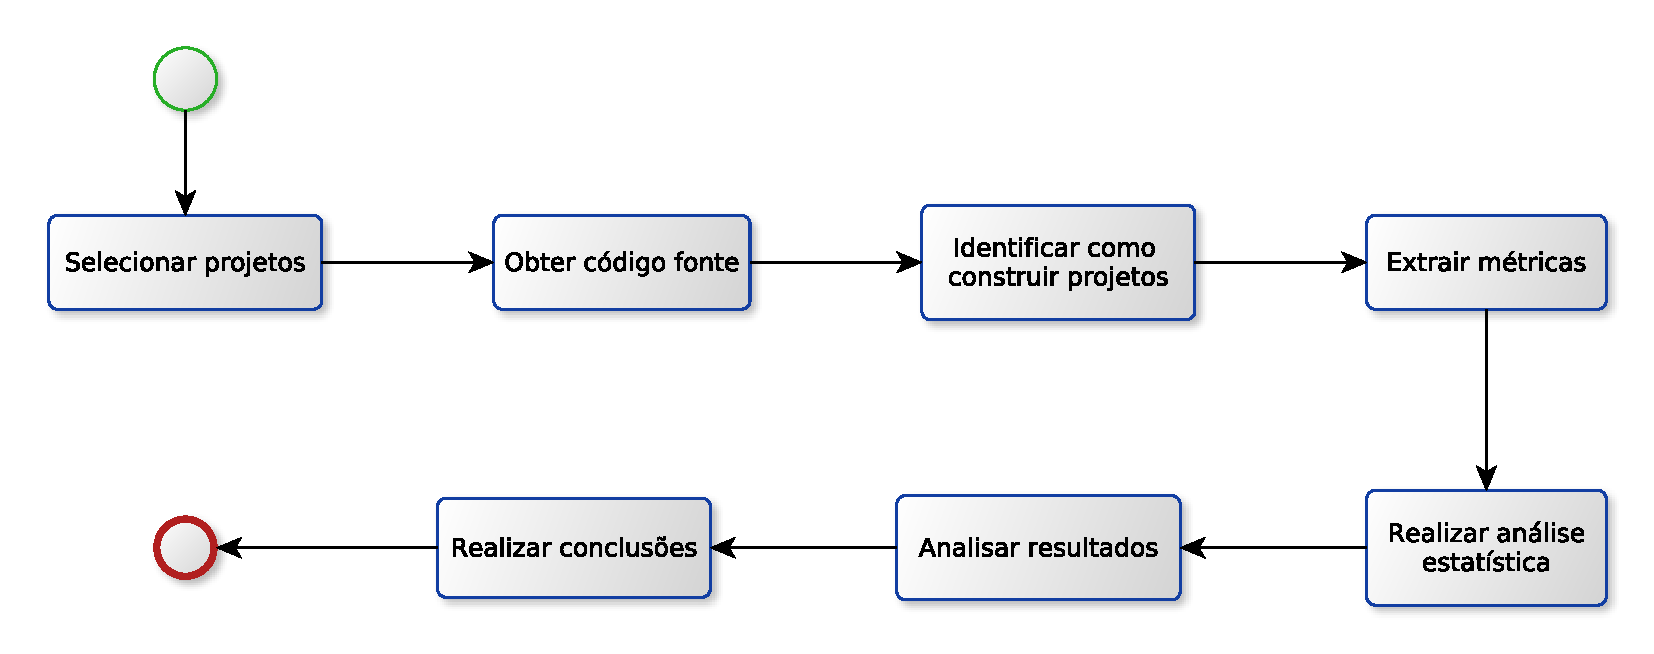
\includegraphics[width=0.8\textwidth]
      {figuras/estudo_de_caso_processo.eps}
  \caption{Processo para execução do estudo de caso}
  \label{processo_estudo_de_caso}
\end{figure}

A seguir a descrição das atividades do processo apresentado no fluxograma \ref{processo_estudo_de_caso}.

\begin{enumerate}\label{desc_processo}
  \item Selecionar projetos de software que atendam os requisitos desse estudo de caso
  \item Obter código fonte dos projetos selecionados
  \item Identificar como construir projetos selecionados 
  \item Executar ferramenta de extração de métricas de vulnerabilidade de código fonte
  \item Realizar análise estatísticas sobre as métricas extraídas, incluindo tratamento dos dados se necessário
  \item Analisar resultados gerados pela análise
  \item Realizar conclusões
\end{enumerate}

Espera-se que esse seja um ciclo completo para execução do estudo de caso proposto, entretanto, é importante salientar que esse
ciclo será executado uma vez, podendo ser alterado no próximo ciclo.

\section{Ferramentas} \label{tools}

A seguir serão apresentadas as ferramentas que serão utilizadas para a realização do estudo de caso definido na seção 
\ref{definicao_estudo} e seguindo a metodologia descrita na seção \ref{metod_estudo}.

\subsection{Analizo} \label{analizo}

Analizo é um conjunto de ferramentas livre, multi-linguagem (C, C++, Java), realiza análise de código fonte de maneira 
extensível e disponibiliza diferentes tipos de visualização. Ele suporta a extração e cálculo de um bom número de métricas de 
código fonte, geração de gráficos de dependência e análise de evolução do software \cite{analizo}.

A seguir as funcionalidades da ferramenta Analizo \footnote{Disponível em http://www.analizo.org/features.html}:

\begin{itemize}
  \item Analisar código-fonte escritos em C, C ++ e Java.
  \item Extrair métricas de código-fonte.
  \item Extrair métricas de uma grande quantidade de projetos em lote (\textit{batch mode}).
  \item Extrair métricas de um repositório.
  \item Desenhar gráfico de dependências.
  \item Analisar evolução do software (analisa-se várias versões do software e uma matriz de evolução é produzida).
\end{itemize}

Será iniciado o processo de manutenção corretiva da funcionalidade de extração de métricas de vulnerabilidade de código fonte 
para as linguagens C e C++, para que melhor atenda as necessidades deste trabalho. Outra funcionalidade que ainda está em 
processo de desenvolvimento é a adição do suporte da linguagem \textit{Perl}.

A ferramenta Analizo é facilmente extensível, desde extratores até formas de visualização. A figura \ref{archanalizo} mostra
como está implementada a arquitetura em camadas da ferramenta \cite{analizoartigo}. Existem basicamente cinco módulos, o 
\textit{Core} é o modulo responsável por atividades centrais como processamento, filtros e modelos por exemplo; 
\textit{Extractor} é o módulo que contém os extratores utilizados, atualmente existem três: \textit{Clang}, \textit{Doxyparse}
e \textit{Sloccount}; \textit{Metrics} é o módulo que contém a lógica para cálculo de todas as métricas, hoje em dia possuindo
37 (trinta e sete) métricas de módulo e 4 (quatro) métricas globais; \textit{Output} é o módulo que será dada a saída da 
ferramenta, atualmente existem opções de banco de dados e arquivo CSV; \textit{Tools} é o módulo que representa várias outras
ferramentas que podem trabalhar tanto acima do \textit{Core} quanto acima dos outros módulos.

\begin{figure}[h]
  \centering
  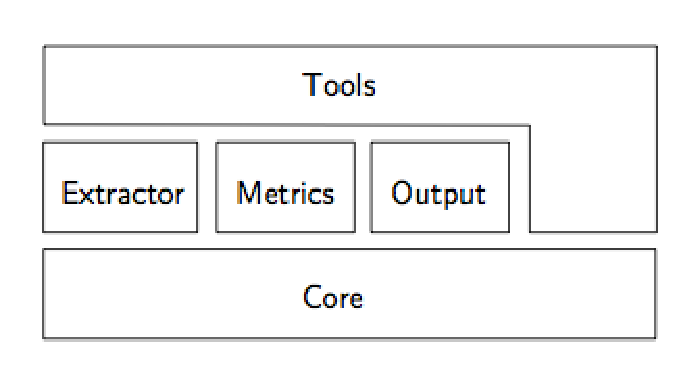
\includegraphics[width=0.5\textwidth]
      {figuras/analizo.eps}
  \caption{Arquitetura da ferramenta Analizo}
  \label{archanalizo}
\end{figure}

\subsection{Clang} \label{clang}

Clang é um compilador \textit{front end} para as linguagens de programação C, C++ e \textit{Objective-C}. O Clang faz parte
do projeto LLVM \textit{Open Source} e utiliza o mesmo comoa seu \textit{back end}. 

O Clang possui algumas funcionalidades e metas disponíveis no seu respectivo \textit{site}\footnote{http://clang.llvm.org}, e
algumas das principais metas são:

\begin{itemize}
  \item Rápida compilação e baixo uso de memória
  \item Diagnóstico expressivos (exemplo, apresentar erros de uma maneira fácil para o usuário)
  \item Compatibilidade com o GCC (\textit{GNU Compiler Collection})
  \item Suportar diversos clientes (exemplo, análise estática e refatoração)
  \item Código fonte base simples e de fácil entendimento ("\textit{hackable}")
\end{itemize}

Algumas dessas metas estão sendo atingidas, por exemplo, em um experimento feito por \cite{naroff2009} evidenciou o rápido
tempo de compilação do Clang em comparação com o GCC. Foi feita a compilação do \textit{PostgreSQL} em computadores com 
configuraçãoes de \textit{hardware} iguais e o resultado obtido é expresso pela figura \ref{clang_gcc}.

\begin{figure}[h]
  \centering
  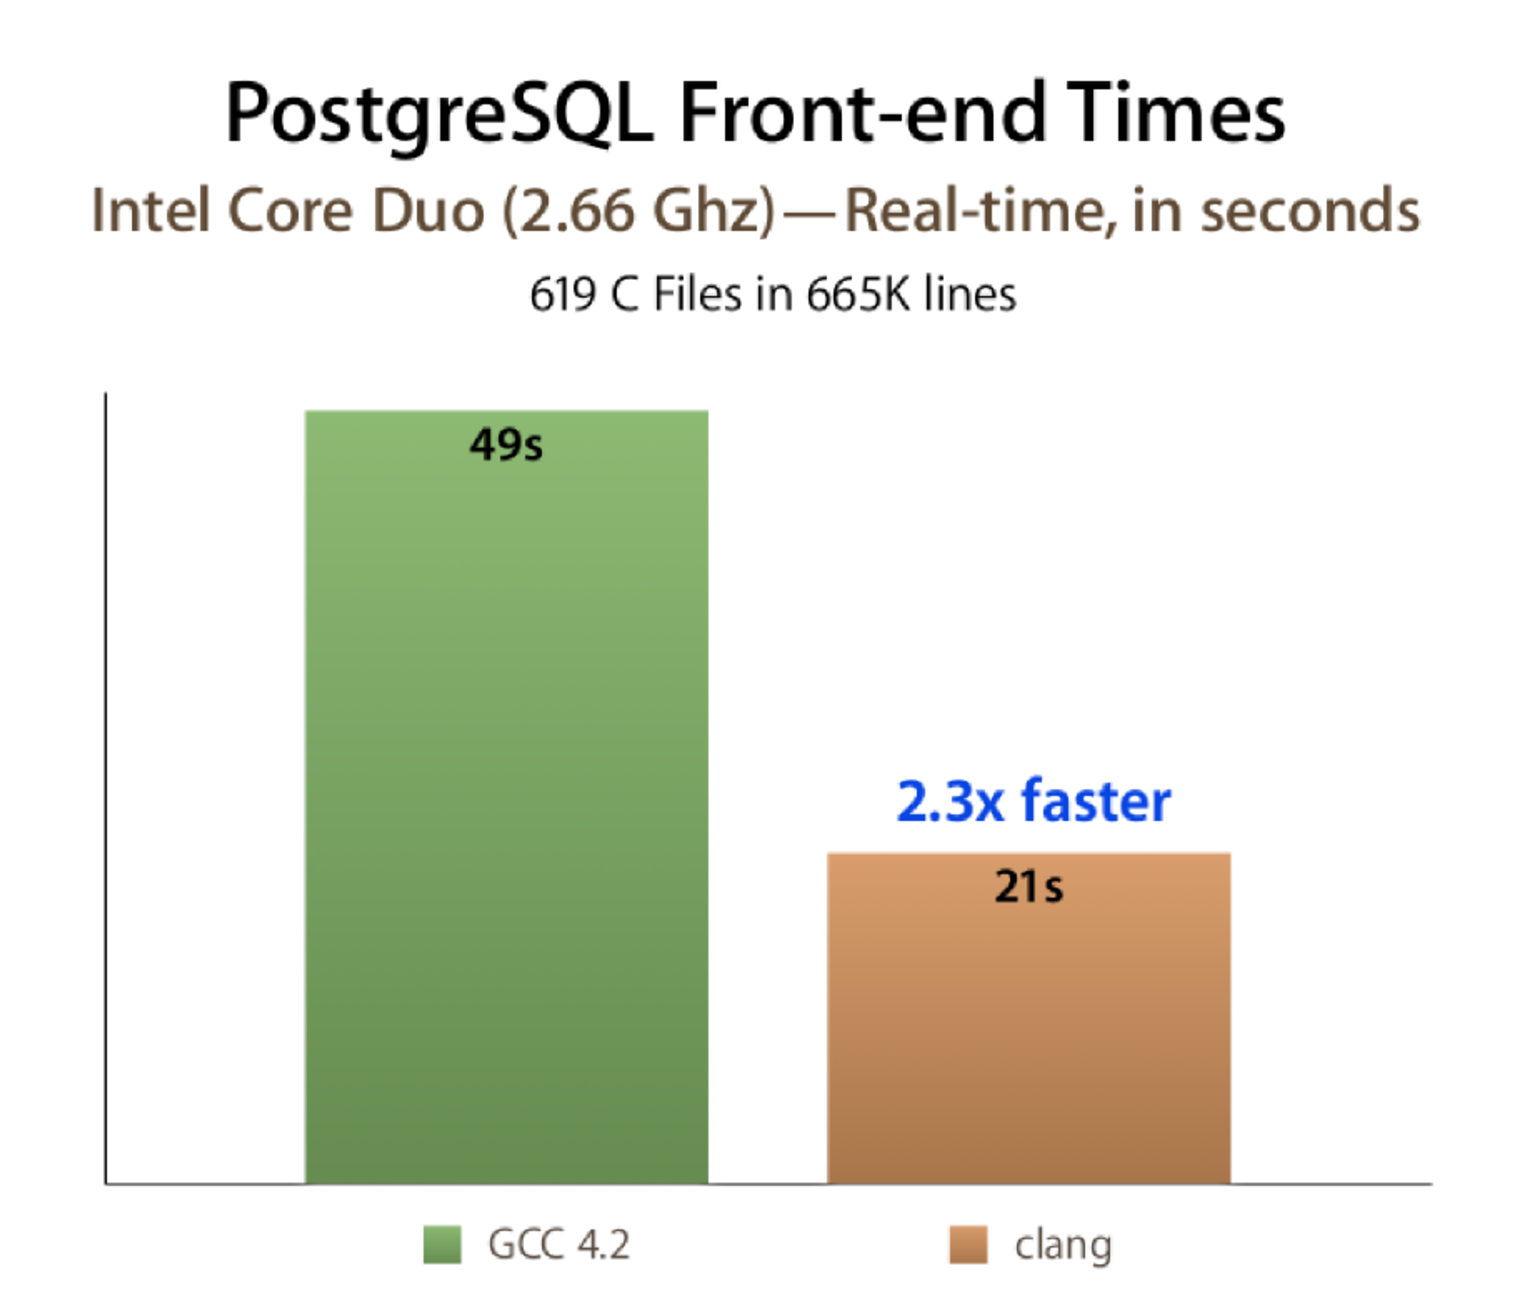
\includegraphics[width=0.4\textwidth]
      {figuras/clang_gcc.eps}
  \caption{Análise de performance do Clang em comparação com o GCC}
  \label{clang_gcc}
\end{figure}

O Clang vem sendo desenvolvido baseado na arquitetura do projeto LLVM, ele possui bibliotecas centrais e bibliotecas de 
aplicativos, conforme é apresentado na figura \ref{clang_arch}. No contexto desse trabalho, o foco é a biblioteca de aplicativo
\textit{Analysis}. A ideia dessa biblioteca é trazer alguns benefícios para os desenvolvedores, como o descobrimento de 
\textit{bugs} o mais cedo possível; checar sistematicamente o código fonte; achar alguns \textit{bugs} mesmo na falta de caso
de testes, no caso de trechos de código difíceis de serem testados \cite{kremenek2009}. 

A análise estática realizada pelo Clang é inter-procedural, podendo achar inconsistências entre funções/métodos, para isso,
é necessária a compilação do código fonte, onde nessa fase será construída a AST (\textit{Abstract Syntaxe Tree})
\cite{kremenek2009}. Essa característica pode não ser muito atraente a primeira vista, pois para realizar a análise do código 
fonte é necessário compila-lo, entretanto, pode ser um ponto positivo tendo em vista que a todo momento que for feita 
construção do software a análise será feita, mesmo que essa questão tenha sido esquecida.

\begin{figure}[h]
  \centering
  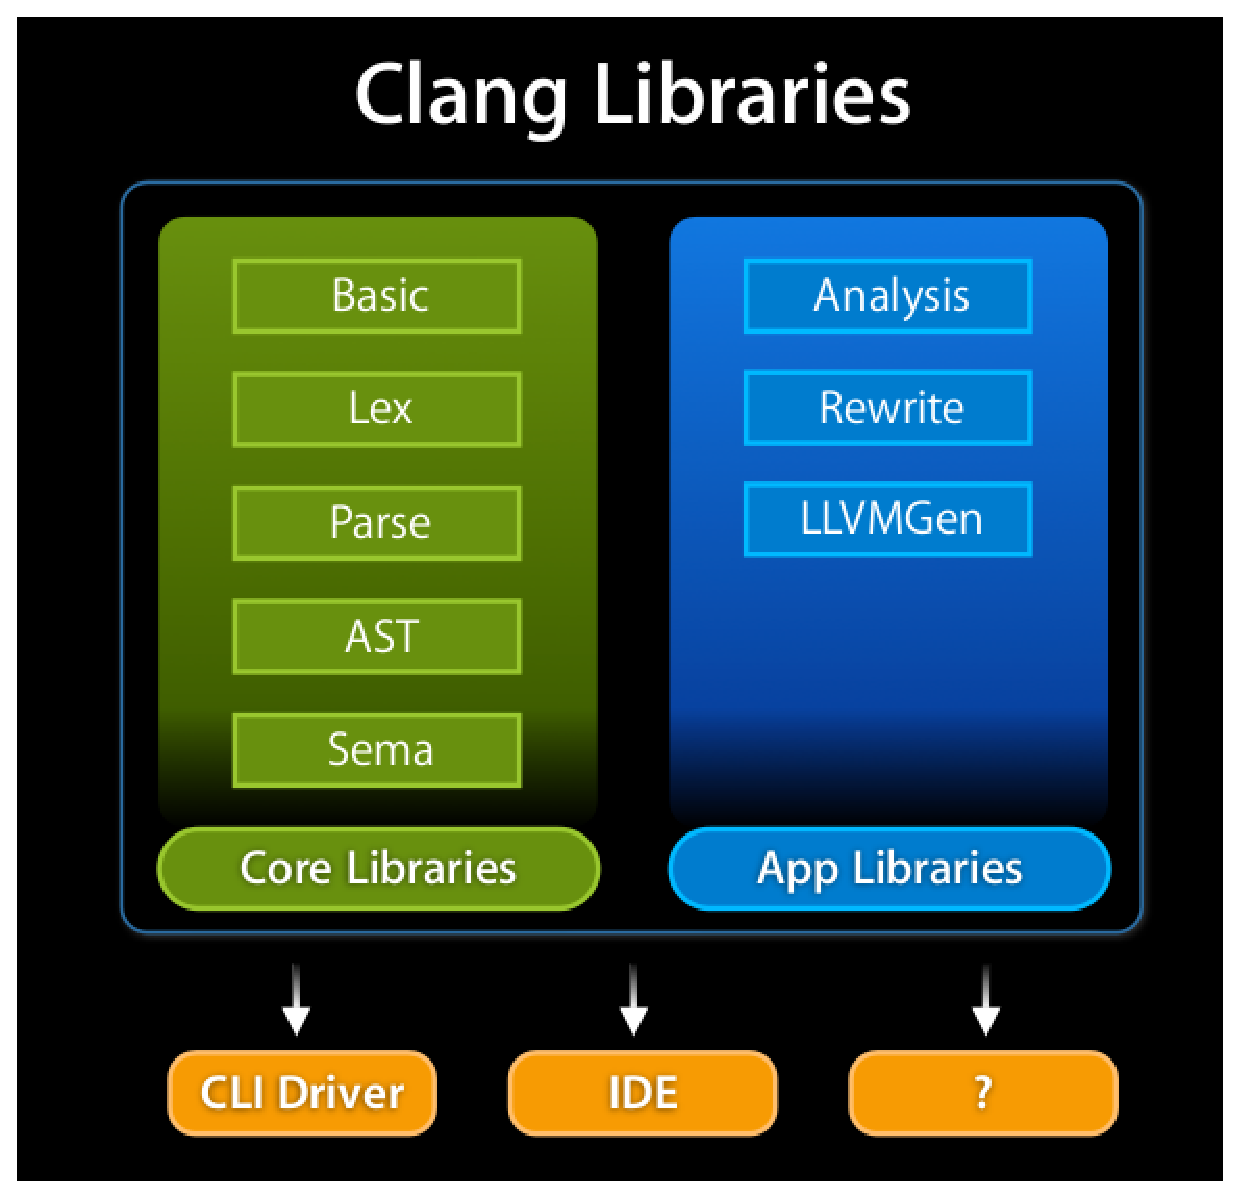
\includegraphics[width=0.4\textwidth]
      {figuras/clang_arch.eps}
  \caption{Arquitetura da ferramenta Clang}
  \label{clang_arch}
\end{figure}

\subsection{\textit{Scripts} para análise estatística} \label{scripts}

Serão utilizados \textit{scripts}\footnote{Disponível em https://gitlab.com/paulormm/tese} em linguagem R
\footnote{http://www.r-project.org/} que foram inicialmente desenvolvidos em \cite{meirelles2013}. Foi escolhida a linguagem R
devido o seu foco e poder para a realiazação de análises estatísticas. O processo de análise estatística que será realizado
por esses \textit{scripts} tentará identificar qual distribuição estatística melhor se encaixa nos dados referentes a 
determinada métrica, são utilizadas as seguintes distribuições estatísticas:

\begin{itemize}
  \item Pareto
  \item Pareto tipo 2
  \item Exponencial
  \item Gama
  \item Weibull
  \item Poison
\end{itemize}

Caso nenhuma das distribuições apresentadas consigam refletir os valores de uma determinada métrica de vulnerabilidade, os
\textit{scripts} tentarão encontrar uma distribuição estatística que melhor se adeque. Gráficos de cada distribuição serão
gerados como saída desse processo de análise estatística para melhor visualização dos dados. Como entrada teremos arquivos
CSV (\textit{Comma Separeted Values}) com os valores das métricas a serem analisadas.

\section{Metodologia} \label{metod_estudo}

Ao iniciar este trabalho havia uma hipótese sobre como deveria se comportar as métricas de vulnerabilidades em projetos de
software livre, baseado no trabalho de \cite{meirelles2013}. A hipótese seria que esse novo tipo de métrica se comportaria
semelhantemente às métricas de design, onde em geral se comportariam como distribuições estatísticas de cauda longa, e com
isso, seria possível analisar os dados e fazer uma avaliação de forma quantitativa. Entretanto, durante o processo empírico
de desenvolvimento deste estudo de caso viu-se que a natureza das métricas são diferentes. As métricas de design em sua grande
maioria possuem valores significativos em todas as suas análises, tendo elas valoração zero ou não, já as métricas de 
vulnerabilidades em grande parte das vezes possuem valoração zero pois não possuem significado, levando em conta que as mesmas
representam a quantidade de cenários de vulnerabilidades presentes no código fonte em questão. Logo, nas métricas de 
vulnerabilidades existirão vários zeros não significativos, atrapalhando uma análise similar a feita em \cite{meirelles2013}.
Tendo isso em vista, decidiu-se então realizar uma análise qualitativa ao invés de quantitativa.

O estudo de caso inicial realizado está seguindo as atividades definidas na seção \ref{definicao_estudo}.

Os requisitos para a seleção dos projetos de software que serão utilizados nesse estudo de caso são:

\begin{itemize}
  \item Possuir uma licensa de software livre (código fonte disponível)
  \item Ser implementado utilizando a(s) linguagem(ns) C e/ou C++
  \item Ser conhecido por sofrer ataques de terceiros devido vulnerabilidades de código fonte
\end{itemize}

O código fonte de cada projeto foi obtido diretamente no site oficial de cada um dos projetos selecionados.

A ferramenta utilizada para extração de métricas de vulnerabilidades foi a Clang (\ref{clang}), entretanto espera-se que seja utilizada
a ferramenta Analizo (\ref{analizo}), sendo essa uma contribuição deste trabalho. E os \textit{scripts} apresentados na seção 
\ref{scripts} foram utilizados para a realização da análise estatística, tendo os dados passados por um processo de adequação do 
formato esperado pelos mesmos, já que o \textit{report} padrão do Clang é um arquivo HTML (\textit{HyperText MarkUp Language}) e os 
\textit{scripts} utilizados esperam como entrada arquivos CSV.

Ao final, como foi dito anteriormente, foi feita uma análise qualitativa dos resultados obtidos, que está apresentado na seção
\ref{analise_estudo}

\section{Análise qualitativa dos resultados obtidos} \label{analise_estudo}

Os projetos selecionados para realizar este estudo de caso foram os seguintes, levando em consideração os requisitos apresentados na
seção \ref{metod_estudo}:

\begin{itemize}
  \item Bash
  \item Firefox
  \item Inetutils
  \item Openssh
  \item Openssl
  \item Python2.7
  \item Ruby-2.1
\end{itemize}



\section{Conclusão}
